\chapter{Model predictive control}
\label{ch:mpc}
In this chapter, the framework conditions of the MPC are described by answering the questions: (i) what is controlled? (ii) How is controlled? (iii) Which curves are controlled? (iii) What data are used? Also, the constraints, the cost function, and the workflow of the MPC script are introduced. The objective of this investigation is to obtain a control signal for the heat pump of the reference building that considers grid services and occupancy comfort. There, the investigation stays in a simulation environment. \newline

\section{Framework conditions of the MPC}
\label{section:FrameworkMPC}
The objective of the MPC is to optimise the control signal of the reference building $\mathbf{u} = (u_1 \enspace u_2)^T = (\dot{Q}_\text{heating} \enspace \dot{Q}_\text{HP})^T$. Thereby, we consider the heat flows of the building in the MPC simulation but, we calculate with a characteristic diagram of the heat pump the electrical control signal $P_\text{HP}$ later. The controlled output is the inside temperature $\mathbf{y} = T_\text{inside}$, which we calculate with the thermal model from \autoref{holeModel}. The desired curves of the $\mathbf{y}$ depend on the presents of occupants, which is determined on an occupancy schedule. Past data of the weather and the dynamic price of the grid $dP$ \nomenclature[P]{dP}{dynamic Price of the grid} is used for the simulation environment. \newline

\textbf{Characteristic diagram of the heat pump:}\newline
    \begin{figure}[h]
            \centering
            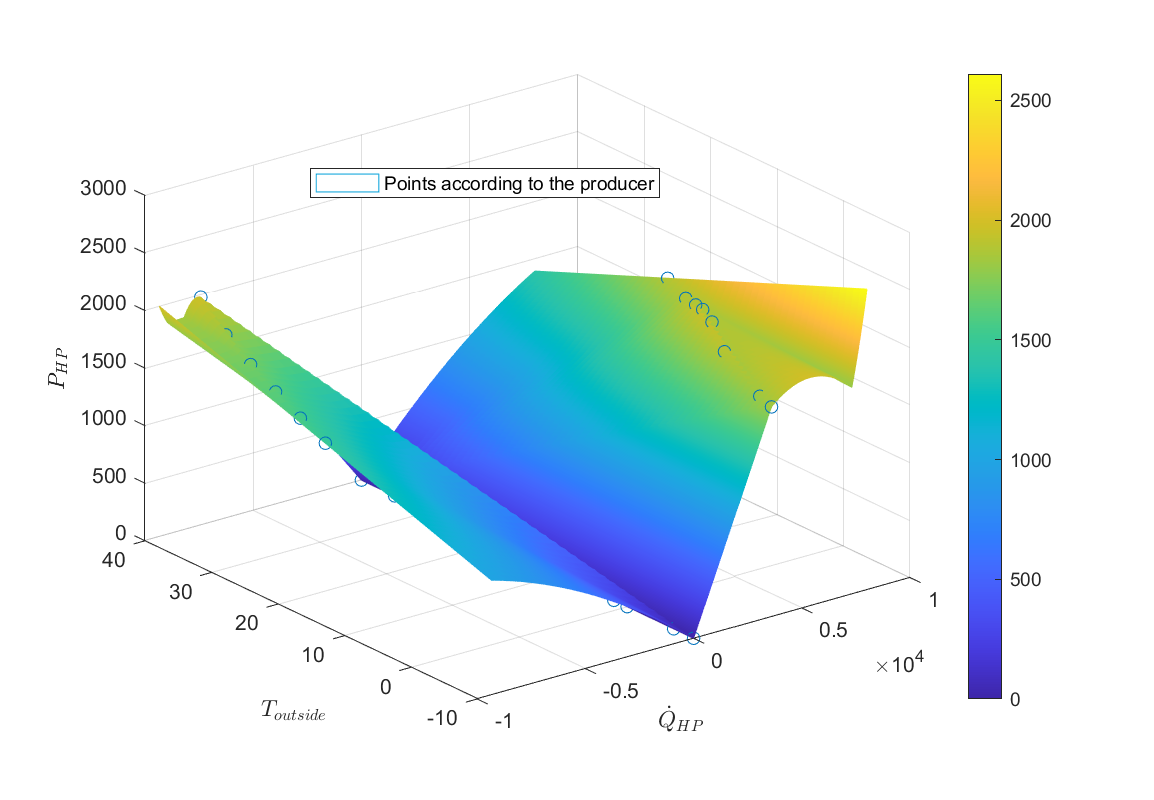
\includegraphics[width=8cm,height=6.5cm]{figure/HeatPumpV55nenn.eps}
           \caption{Interpolation of the characteristic diagram of the heat pump with the heating inlet temperature of 55°C and nominal power according to \cite{TUM}}
           \label{fig:HeatpumpKennfeld}
    \end{figure}
    
\textbf{Occupancy schedule:}\newline
    \begin{figure}[h]
            \centering
            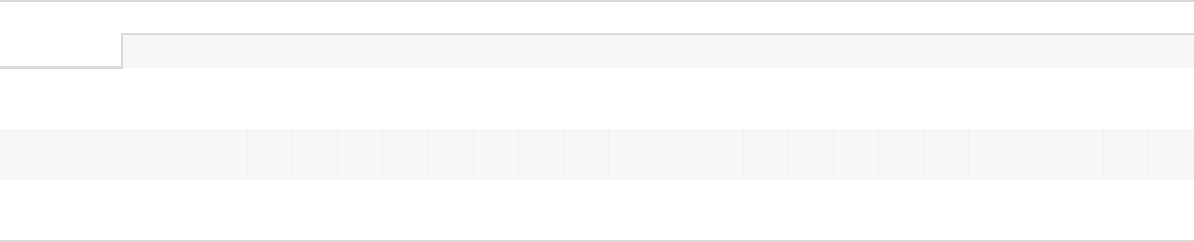
\includegraphics[]{figure/Occupancy_schedule.pdf_tex}
           \caption{Occupancy schedule of the reference building}
           \label{fig:OccupancySchedule}
    \end{figure}

\textbf{Past data:}\newline

\section{The Constraints}
\label{section:theconstraints}
\section{The Cost function}
\label{section:thecostfunction}
\begin{equation}
    \text{minimize} \sum_{k=1}^{N-1} w_\text{1}\cdot (y-y_\text{track})^2 + w_\textbf{2}\cdot(u_\text{2}\cdot dP)^2 + w_\text{3} \cdot \eta^2
\end{equation}
\section{Workflow of the MPC script}
\label{section:workflowMPC}
\begin{figure}[h]
            \centering
            \def\svgwidth{0.6\textwidth}
            \input{figure/workflowMPC.pdf_tex}
            \caption{Workflow of the MPC script}
            \label{fig:workflowMPC}
    \end{figure}